\documentclass[12pt, a4paper]{scrreprt}

%% Language and font encodings
\usepackage[ngerman]{babel}
\usepackage[utf8]{inputenc}
\usepackage[T1]{fontenc}
\usepackage{helvet}
\renewcommand{\familydefault}{\sfdefault}
\usepackage{bibgerm}

%% Sets page size and margins
\usepackage[a4paper,top=2.5cm,bottom=2cm,left=2cm,right=2cm]{geometry}

%% Useful packages
\usepackage{amsmath}
\usepackage{graphicx}
\usepackage[colorlinks=true, allcolors=blue]{hyperref}
\usepackage{listings}
\usepackage{subcaption}

\lstset{
    basicstyle=\linespread{1.1}\ttfamily\footnotesize,
    breaklines=true,                 
    numbers=left,                    
    numbersep=5pt,                  
    showspaces=false,                
    showstringspaces=false,
    showtabs=false,                  
    tabsize=2,
    extendedchars=true,
    literate={ä}{{\"a}}1 {ö}{{\"o}}1 {ü}{{\"u}}1 {Ä}{{\"A}}1 {Ö}{{\"O}}1 {Ü}{{\"U}}1 {ß}{{\ss}}1 {€}{{\EUR}}1
}

%% tcolorbox
\usepackage{tcolorbox}
\definecolor{mycolor}{rgb}{0.122, 0.435, 0.698}% Rule colour

\setlength{\parindent}{0em}
\setlength{\parskip}{1em}

\usepackage{scrlayer-scrpage}
\KOMAoptions{
  headwidth=\textwidth+30pt:-15pt,
  headsepline=.2pt
}
%\clearpairofpagestyles
\ihead{Mr. Trash Design Dokument}
\chead{TU Wien, MSE}
\ohead{Hurbean, Schweiger [Gruppe 06]}
\renewcommand\chapterpagestyle{scrheadings}


\title{\vspace{-1cm}Mr. Trash}
\subtitle{App zur effizienten Müllentsorgung}
\author{
    Hurbean, Alexander\\
    \texttt{e01625747}
    \and
    Schweiger, Philipp\\
    \texttt{e01634254}}
\titlehead{\centering
\includegraphics[width=\textwidth]{../graphical/icon/4x/ic_material_product_icon_192pxxxxhdpi.png}}


\begin{document}
\maketitle

\null\vfill
\noindent
App Design Document\\ 
Mobile (App) Software Engineering\\
Technische Universität Wien\\
Version v1.1, März 2019
\newpage

\tableofcontents

% ______________________
% Kapitel Konzept
% ______________________
\chapter{Konzept}

\section{Geplanter Name der App}
Der gewählte Name der App ist Mr. Trash. Die Idee dahinter ist, dass der Name leicht zu merken ist und der User somit sich leicht merken kann "wen er fragen kann", wenn er/sie wissen will, "wohin mit dem Müll".

Weiters lässt sich dazu ein passendes Logo ableiten, dass schlicht ist und davon zeugt, dass die App die richtige sei, wenn es um Fragen im Themenbereich Müll geht.

\section{Kurzbeschreibung}
Mr.Trash ermöglicht es dem unerfahrenen Mülltrenner effizient den richtigen Ort, seinen Müll zu entsorgen, in seiner Nähe zu finden oder einfach um zu sehen ob es ok ist, diesen Müll im Haushaltsmüll zu entsorgen. Die App stellt sicher, dass nie wieder Müll falsch entsorgt wird und somit Umweltfreundlichkeit gewährleistet wird und der Nutzer möglichst wenig Zeit und Know-How benötigt um Müll richtig zu trennen.

Ganz nützlich ist die App für das Auffinden spezieller, zeitlich bedingt vorhandener, "Mobilen Problemstoffsammelstellen", die ebenfalls, samt verfügbaren Uhrzeiten, angezeigt werden.

Nach dem Starten der App, ist es dem User sofort möglich ein Produkt aus einer ausführlichen Liste (auch verfügbar unter wien.gv.at~\cite{muelltrennabc}) auszuwählen. Alternativ dazu kann er auch einfach die Suche im oberen Bereich zu nutzen um das gewünschte Produkt zu finden.

Sobald das zu entsorgende Produkt gefunden wurde, wird der User durch anklicken zu einem neuen Schirm geführt, wo ersichtlich ist, wie er sein Produkt entfernen kann. Wenn vorhanden, können durch einen Klick auf den rechten unteren Text in der Card die nahesten Orte (z.B. Mistplatz) auf einer Google Maps Karte angezeigt werden.

Alternativ dazu, kann der User auch den Floating Button rechts unten nutzen, um einfach die nahesten korrekten Orte zur Müllentsorgung auf einer Karte angezeigt zu bekommen (unabhängig von Entsorgungsortart).

\section{Beschreibung der gewählten Datensätze}
\subsection{Sämtliche Müll-Daten Wien  \cite{alleMuell}}
    Hier sind die gesamten (bis auf die Öffnungszeiten) Daten die wir nutzen in einem Sammellink. Alle sind mit dem Tag "Müll" versehen und haben eine Vielfalt an Formaten, unter anderem JSON.
\subsection{Problemstoffsammelstelle Wien \cite{problemstoffsammelstellen}}
    Dieser Datensatz beschreibt alle Problemstoffsammelstellen in Wien.

    Die Daten wurden letztens am 18.03.2019 um 15:40:14 Uhr aktualisiert und sind somit aktuell.

    Das Format ist:
    \begin{tcolorbox}
        BEZIRK: Wiener Gemeindebezirksnummer\\
        ADRESSE: Adresse (Straßenname, Orientierungsnummer)\\
        OEFFNUNGSZEIT: Öffnungszeiten (Wochentag, Uhrzeit)\\
        ANMERKUNG: Zusatzinformation (dezentrale Prosa/zukünftige Prosa\\
        TELEFON: Telefonnummer\\
        WEITERE\_INFORMATION: Hyperlink 
    \end{tcolorbox}
    
    Ein Beispieldatensatz wäre:
    \begin{lstlisting}
"type": "Feature",
"id": "PROBLEMSTOFFOGD.508705",
"geometry": {
    "type": "Point",
    "coordinates": [
        16.400549599361053,
        48.18605159964703
    ]
},
"properties": {
    "BEZIRK": 3,
    "ADRESSE": "Grasbergergasse 3",
    "OEFFNUNGSZEIT": "Montag bis Samstag (werktags) von 7:00 bis 18:00 Uhr",
    "ANMERKUNG": "Mistplatz - Prosa",
    "TELEFON": "(01) 546 48",
    "WEITERE_INFORMATION": "http://www.wien.gv.at/umwelt/ma48/entsorgung/problemstoffsammlung/",
    "SE_SDO_ROWID": 508705,
    "SE_ANNO_CAD_DATA": null
}
    \end{lstlisting}
\subsection{Altstoffsammelstelle Wien \cite{alstoffsammelstellen}}
    Dieser Datensatz beschreibt alle Altstoffsammelstellen in Wien.

    Die Daten wurden letztens am 18.03.2019 um 12:12:34 Uhr aktualisiert und sind somit aktuell.

    Das Format ist:
    \begin{tcolorbox}
        BEZIRK: Wiener Gemeindebezirksnummer\\
        STRASSE: Straßenname gem. amtlichem Straßennamenverzeichnis\\
        BEZUG: Adressbezug\\
        ONR: Orientierungsnummer gem. Wiener Adressregister\\
        FRAKTION\_PA: Papier (Flag)\\
        FRAKTION\_BI: Biomüll (Flag)\\
        FRAKTION\_DO: Altmetall (Flag)\\
        FRAKTION\_G: Altglas (Flag)\\
        FRAKTION\_KV: Kunststoff (Flag)\\
        URL\_TEXT: Hyperlink
    \end{tcolorbox}
    
    Ein Beispieldatensatz wäre:
    \begin{lstlisting}
"type": "Feature",
"id": "ALTSTOFFSAMMLUNGOGD.2518868",
"geometry": {
    "type": "Point",
    "coordinates": [
        16.362475582469685,
        48.15935192124853
    ]
},
"geometry_name": "SHAPE",
"properties": {
    "BEZIRK": 10,
    "STRASSE": "Sibeliusstraße",
    "BEZUG": "vor",
    "ONR": "8",
    "BIS": null,
    "STIEGE": null,
    "FRAKTION_PA": 0,
    "FRAKTION_BI": 1,
    "FRAKTION_DO": 1,
    "FRAKTION_G": 1,
    "FRAKTION_KV": 1,
    "FRAKTION_TEXT": " Kunststoff, Altmetall, Altglas, Biomüll",
    "URL_TEXT": "http://www.wien.gv.at/umwelt/ma48/beratung/muelltrennung/index.html",
    "SE_SDO_ROWID": 2518868,
    "SE_ANNO_CAD_DATA": null
    \end{lstlisting}
\subsection{Mistplätze Standorte Wien \cite{mistplaetze}}
    Dieser Datensatz beschreibt alle Mistplätze in Wien.

    Die Daten wurden letztens am 18.03.2019 um 12:11:51 Uhr aktualisiert und sind somit aktuell.

    Das Format ist:
    \begin{tcolorbox}
        BEZIRK: Wiener Gemeindebezirksnummer\\
        ADRESSE: Adresse (Straßenname, Orientierungsnummer)\\
        OBJEKT: Objekttyp\\
        OEFFNUNGSZEIT: Öffnungszeit (Wochentag, Uhrzeit)
    \end{tcolorbox}
    
    Ein Beispieldatensatz wäre:
    \begin{lstlisting}
"type": "Feature",
"id": "MISTPLATZOGD.824127",
"geometry": {
    "type": "Point",
    "coordinates": [
        16.367822851014218,
        48.25480470125357
    ]
},
"geometry_name": "SHAPE",
"properties": {
    "BEZIRK": 19,
    "ADRESSE": "Grinzinger Straße 151",
    "OBJEKT": "WD/Mistplatz",
    "OEFFNUNGSZEIT": "Mo-Sa 7:00-18:00 Uhr",
    "SE_SDO_ROWID": 824127,
    "SE_ANNO_CAD_DATA": null
}
    \end{lstlisting}
\subsection{Mobile Problemstoffsammelstelle Standorte Wien \cite{mobileProblemstoffsmst}}
    Dieser Datensatz beschreibt alle Problemstoffsammelstellen in Wien.

    Die Daten wurden letztens am 18.03.2019 um 11:56:58 Uhr aktualisiert und sind somit aktuell.

    Das Format ist:
    \begin{tcolorbox}
        BEZIRK: Wiener Gemeindebezirksnummer\\
        ADRESSE: Adresse (Straßenname, Orientierungsnummer)\\
        OBJEKT: Objekttyp\\
        OEFFNUNGSZEIT: Öffnungszeit (Wochentag, Uhrzeit) 
    \end{tcolorbox}
    
    Ein Beispieldatensatz wäre:
    \begin{lstlisting}
"type": "Feature",
"id": "MISTPLATZOGD.824279",
"geometry": {
    "type": "Point",
    "coordinates": [
        16.30411114330886,
        48.16070475694853
    ]
},
"geometry_name": "SHAPE",
"properties": {
    "BEZIRK": 12,
    "ADRESSE": "Wundtgasse/Jägerhausgasse",
    "OBJEKT": "WD/Mistplatz",
    "OEFFNUNGSZEIT": "Mo-Sa 7:00-18:00 Uhr",
    "SE_SDO_ROWID": 824279,
    "SE_ANNO_CAD_DATA": null
}
    \end{lstlisting}
\subsection{Christbaumsammelstellen Wien \cite{christbaumsammelstellen}}
    Dieser Datensatz beschreibt alle Christbaumsammelstellen in Wien.

    Die Christbaumsammelstellen wurden am 01.03.2019 11:21:09 entfernt und sind somit aktuell.

    Das Format ist:
    \begin{tcolorbox}
        BEZIRK: Wiener Gemeindebezirksnummer\\
        ADRESSE: Adresse (Bezirksnummer, Straßenname, Orientierungsnummer)\\
        GEÖFFNET VON: Beginn der Öffnungszeit (Tag)\\
        GEÖFFNET BIS: Ende der Öffnungszeit (Tag) 
    \end{tcolorbox}
    
    Da es derzeit keine Christbaumsammelstellen gibt, git es auch keine Daten dazu.
\subsection{Mülltrenn ABC \cite{muelltrennabc}}
Diese Daten Nutzen wir um dem User richtige Orte vorzuschlagen, wo er seinen Müll entsorgen kann, abhängig von was er gerade entsorgen will. Dazu brauchen ist eine möglichst ausführliche Liste nötig, mit verschiedensten Müllarten, damit der User fündig wird, wenn er eingibt was er entsorgen will.

Zum beschaffen dieser JSON Daten wurde ein selbst geschriebener Python Web Scraper auf dem angegebenen Link ausgeführt. Die Daten sind auf den letzten Stand (laut wien.gv.at), da diese direkt von der Webseite geholt werden.

Das Skript sieht wie folgt aus:

\lstinputlisting{scrape.py}

Ein Ausschnitt aus der generierten JSON-Datei sieht wie folgt aus:

\begin{lstlisting}
"B": {
"Babywindeln": [
    "Restmülltonne",
    "Mistplatz"
],
"Backrohrreiniger": [
    "Problemstoffsammelstelle",
    "Mistplatz"
],
"Batterien bis 5 kg": [
    "Fachhandel",
    "Problemstoffsammelstelle",
    "Mistplatz"
], 
\end{lstlisting}

\section{Wireframes}
\begin{figure}[h]
\centering
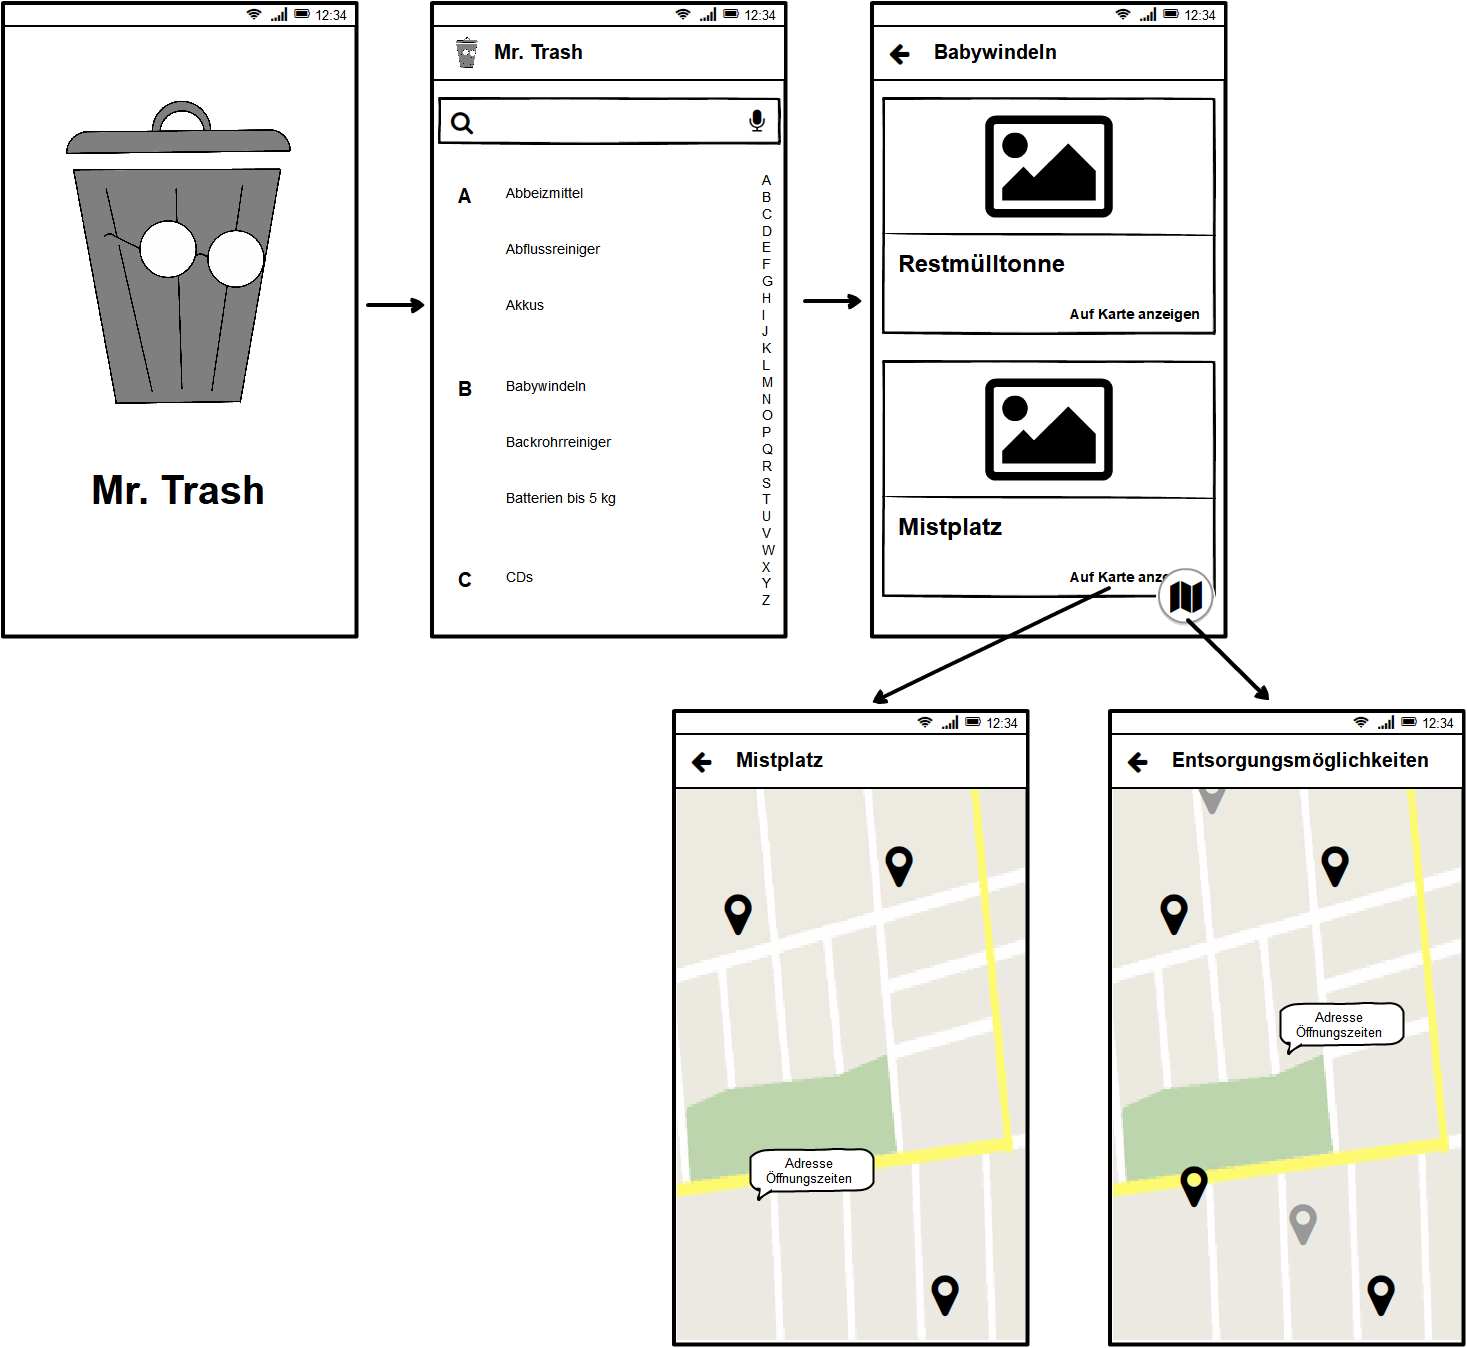
\includegraphics[width=16cm]{../graphical/wireframes.png}
\caption{\label{fig:art1} Wireframes}
\end{figure}

\subsection{Beschreibung}
Mr. Trash gliedert sich in 5 verschiedene Screens. Beim Start der App sieht man den Splash-Screen mit Logo und Namen der App. \\
Ist der Ladevorgang beendet gelangt man zum Main-Screen der App. Dabei handelt es sich um eine Liste aller unterstützen Müllarten. Auf dieser Seite wird ein Auto-Complete-Suchfeld angeboten, um schneller die gewünschte Müllart zu finden. Zusätzlich wird auf der rechten Seite eine Buchstaben-Scrollbar angeboten.\\
Klickt man nun auf eine Müllart, werden am nächsten Screen die Arten der Entsorgungsmöglichkeiten angezeigt. Diese werden als Liste von Cards dargestellt. Eine Card enthält ein Bild, als Titel die Art der Entsorgungsmöglichkeit und einen Button, welcher in weiterer Folge eine Map mit allen Standorten dieser Art anzeigt. Des Weiteren befindet sich ein Floating-Button rechts unten am Screen, um eine Map mit den Standorten aller Entsorgungsmöglichkeiten, für diese Müllart, anzuzeigen.\\
Klickt man auf der Map auf einen der Standorte, werden Adresse und Öffnungszeiten angezeigt.

\newpage

% ______________________
% Kapitel Graphischer Entwurf
% ______________________

\chapter{Graphischer Entwurf} 

\section{High-Fidelity Mockup}
\begin{figure}[h]
\centering
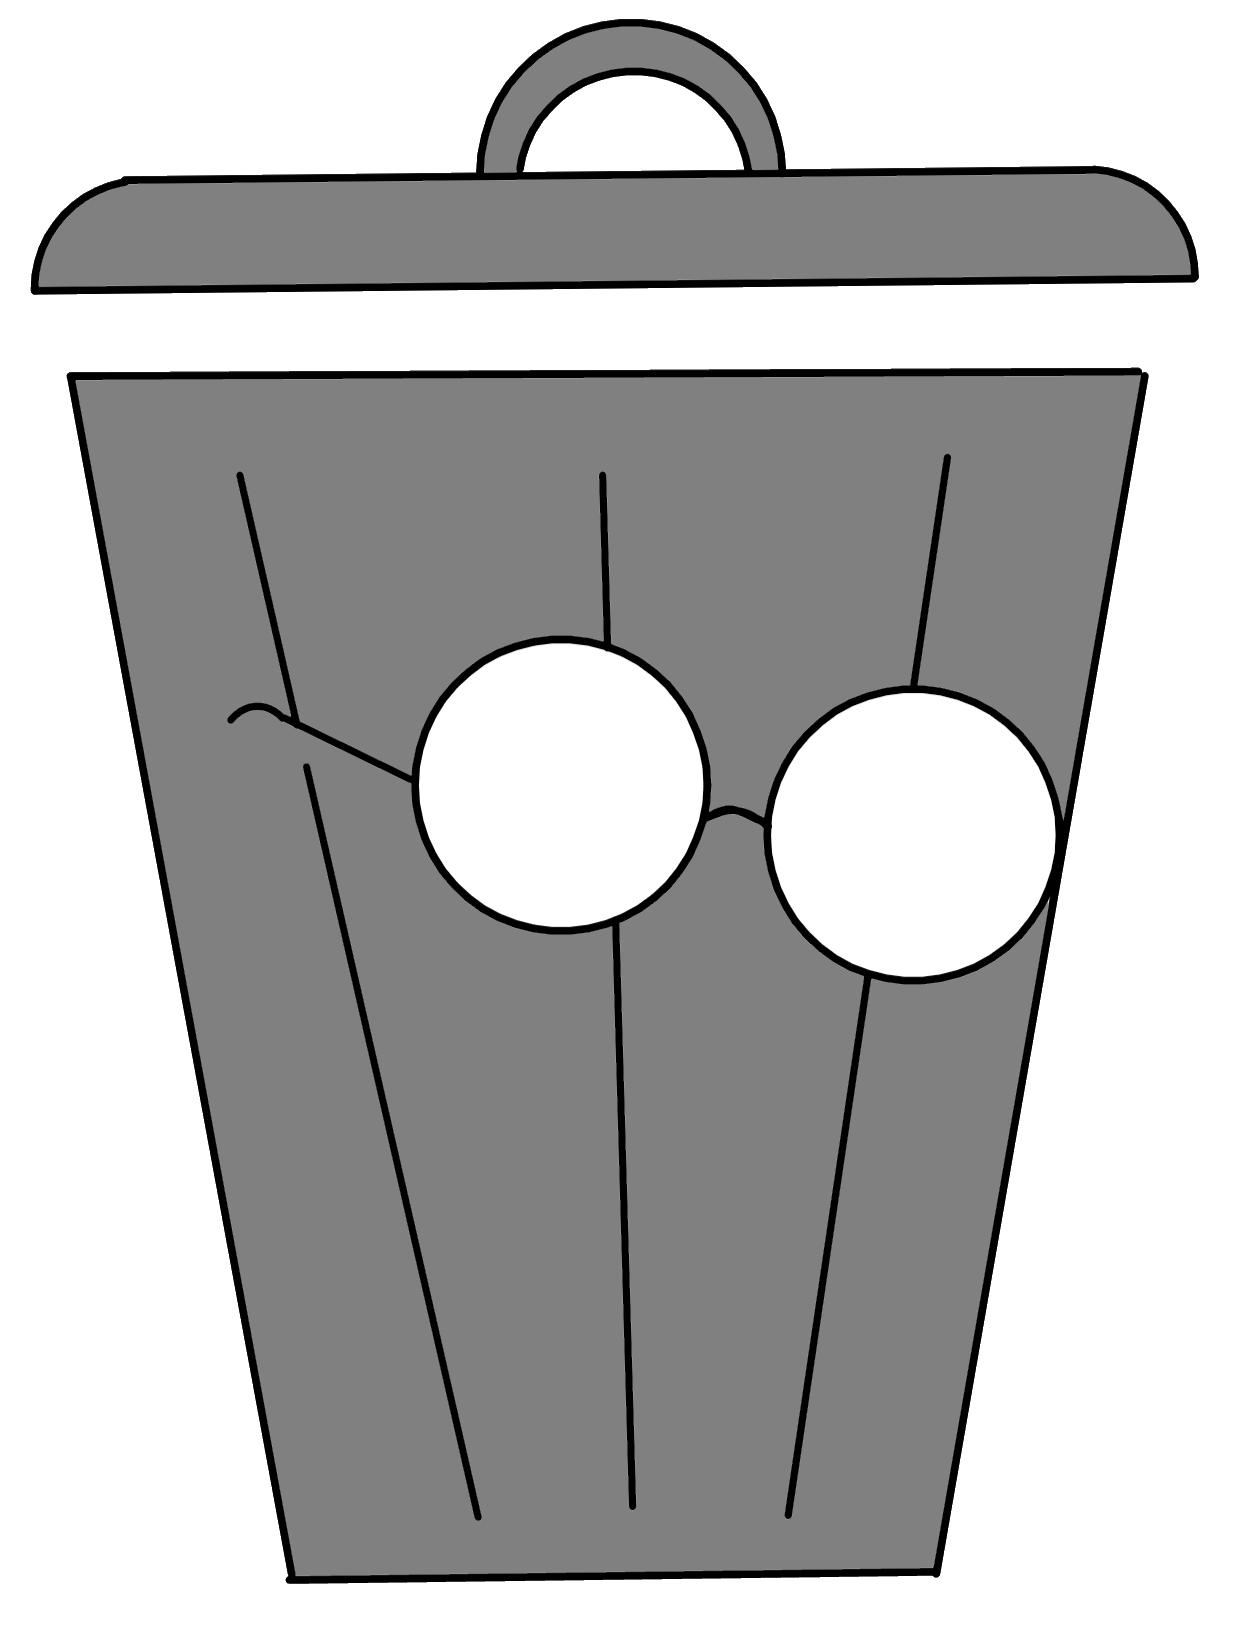
\includegraphics[width=0.3\textwidth]{../graphical/drafts/logo_draft_color.png}
\caption{\label{fig:art1} Art example}
\end{figure}

\newpage
\section{Product Icon}

Das Product Icon stellt einen stylisierten Mistkübel da, der eine Brille auf hat. Dies soll auch das Mascottchen der App sein, Mr.Trash, der sich mit den Müllproblemen des Users auskennt und ihm dabei hilft, seinen Müll zu trennen.

Das Logo wurde nach den Guidelines von Googles Material Design~\cite{materialproductguideline} mit Adobe Illustrator CC~\cite{adobeillustrator} und dem Adobe Illustrator Product Icon Template~\cite{stickersheets} von Google erstellt.

\begin{figure}[h]
\centering
\begin{subfigure}{.3\textwidth}
  \centering
  
\includegraphics[width=.1875\linewidth]{../graphical/icon/0.75x/ic_material_product_icon_192pxldpi.png}
  \caption{0.75x | low density}
  \label{fig:075}
\end{subfigure}%
\begin{subfigure}{.3\textwidth}
  \centering
  
\includegraphics[width=0.25\linewidth]{../graphical/icon/1x/ic_material_product_icon_192pxmdpi.png}
  \caption{1x | medium density}
  \label{fig:1}
\end{subfigure}%
\begin{subfigure}{.3\textwidth}
  \centering
  
\includegraphics[width=0.375\linewidth]{../graphical/icon/1.5x/ic_material_product_icon_192pxhdpi.png}
  \caption{1.5x | high density}
  \label{fig:15}
\end{subfigure}%
\\
\begin{subfigure}{.5\textwidth}
  \centering
  
\includegraphics[width=0.375\linewidth]{../graphical/icon/2x/ic_material_product_icon_192pxxhdpi.png}
  \caption{2x | extra high density}
  \label{fig:2}
\end{subfigure}%
\begin{subfigure}{.5\textwidth}
  \centering
  
\includegraphics[width=.5\linewidth]{../graphical/icon/3x/ic_material_product_icon_192pxxxhdpi.png}
  \caption{3x | extra extra high density}
  \label{fig:3}
\end{subfigure}%
\\
\begin{subfigure}{\textwidth}
  \centering
  
\includegraphics[width=.375\linewidth]{../graphical/icon/4x/ic_material_product_icon_192pxxxxhdpi.png}
  \caption{4x | extra extra extra high density}
  \label{fig:4}
\end{subfigure}%
\caption{Auflösungen des App-Icons}
\label{fig:aufl}
\end{figure}

\bibliographystyle{abbrv}
\bibliography{references}

\end{document}